\documentclass{standalone}
\usepackage{tikz}
\usetikzlibrary{patterns, positioning}


\begin{document}
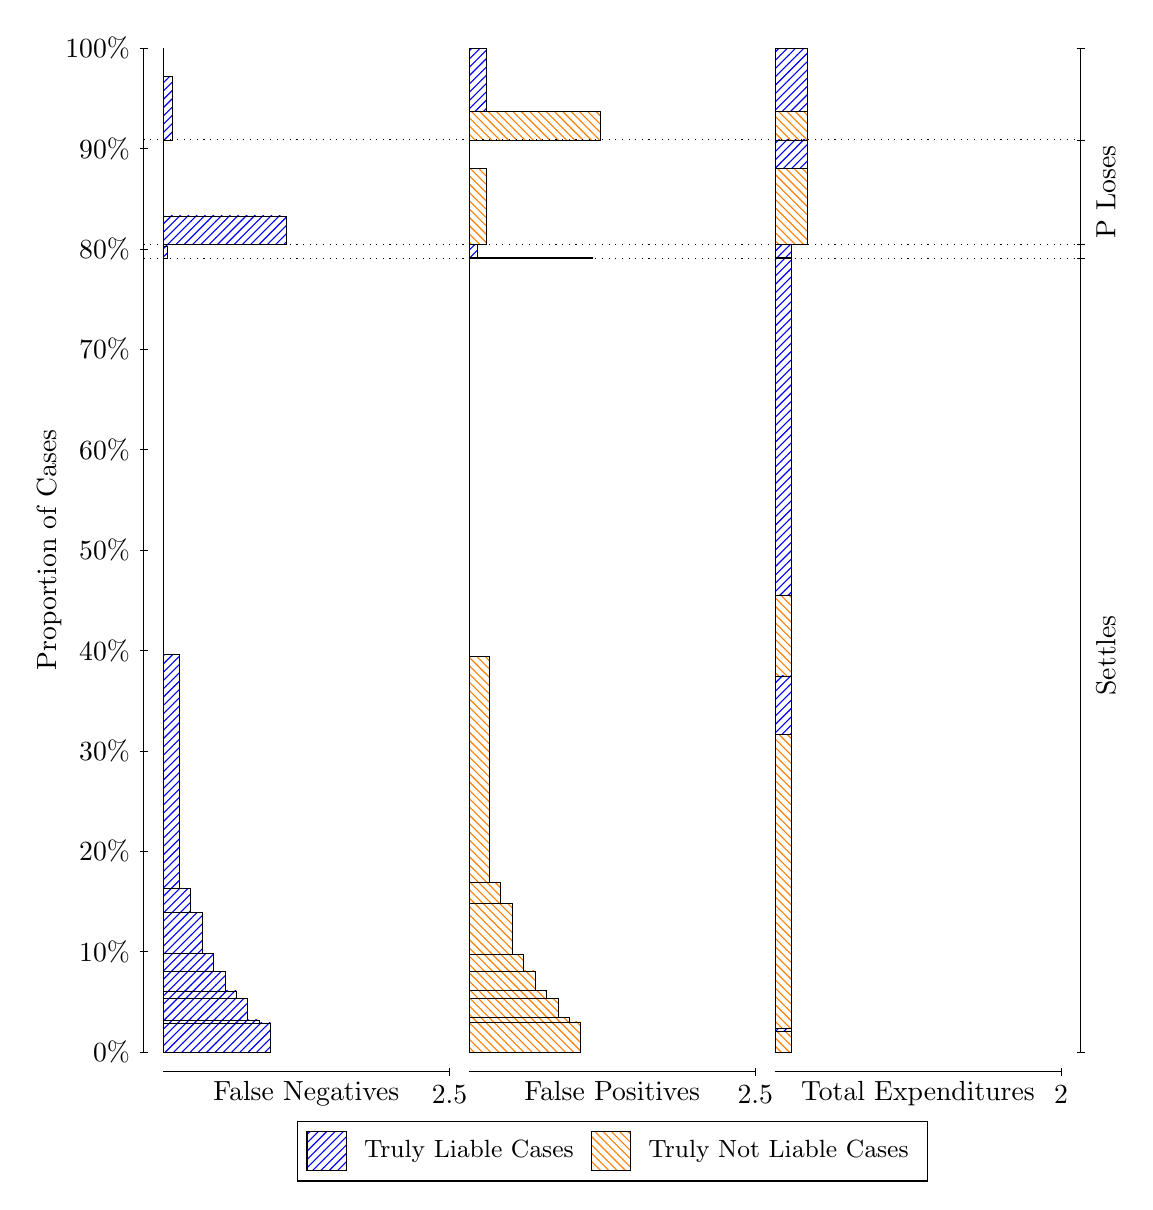
\begin{tikzpicture}
\draw[black, very thin] (1.5,1.75) -- (1.5,14.5);
\node[rotate=90, text=black, anchor=center] at (0.3, 8.125) {Proportion of Cases};
\draw[black, very thin] (1.45,1.75) -- (1.55,1.75);
\node[text=black, anchor=east] at (1.45, 1.75) {0\%};
\draw[black, very thin] (1.45,3.025) -- (1.55,3.025);
\node[text=black, anchor=east] at (1.45, 3.025) {10\%};
\draw[black, very thin] (1.45,4.3) -- (1.55,4.3);
\node[text=black, anchor=east] at (1.45, 4.3) {20\%};
\draw[black, very thin] (1.45,5.575) -- (1.55,5.575);
\node[text=black, anchor=east] at (1.45, 5.575) {30\%};
\draw[black, very thin] (1.45,6.85) -- (1.55,6.85);
\node[text=black, anchor=east] at (1.45, 6.85) {40\%};
\draw[black, very thin] (1.45,8.125) -- (1.55,8.125);
\node[text=black, anchor=east] at (1.45, 8.125) {50\%};
\draw[black, very thin] (1.45,9.4) -- (1.55,9.4);
\node[text=black, anchor=east] at (1.45, 9.4) {60\%};
\draw[black, very thin] (1.45,10.675) -- (1.55,10.675);
\node[text=black, anchor=east] at (1.45, 10.675) {70\%};
\draw[black, very thin] (1.45,11.95) -- (1.55,11.95);
\node[text=black, anchor=east] at (1.45, 11.95) {80\%};
\draw[black, very thin] (1.45,13.225) -- (1.55,13.225);
\node[text=black, anchor=east] at (1.45, 13.225) {90\%};
\draw[black, very thin] (1.45,14.5) -- (1.55,14.5);
\node[text=black, anchor=east] at (1.45, 14.5) {100\%};

\draw[black, very thin] (13.4,1.75) -- (13.4,14.5);
\draw[black, very thin] (13.35,1.75) -- (13.45,1.75);
\node[anchor=west] at (13.35, 1.75) {};
\draw[black, very thin] (13.35,11.824) -- (13.45,11.824);
\node[anchor=west] at (13.35, 11.824) {};
\draw[black, very thin] (13.35,12.006) -- (13.45,12.006);
\node[anchor=west] at (13.35, 12.006) {};
\draw[black, very thin] (13.35,13.334) -- (13.45,13.334);
\node[anchor=west] at (13.35, 13.334) {};
\draw[black, very thin] (13.35,14.5) -- (13.45,14.5);
\node[anchor=west] at (13.35, 14.5) {};

\draw[black, very thin, pattern color=blue, pattern=north east lines] (1.75,1.75) rectangle (3.1125,2.1199);
\draw[black, very thin, pattern color=blue, pattern=north east lines] (1.75,2.1199) rectangle (2.9672,2.1562);
\draw[black, very thin, pattern color=blue, pattern=north east lines] (1.75,2.1562) rectangle (2.8218,2.4354);
\draw[black, very thin, pattern color=blue, pattern=north east lines] (1.75,2.4354) rectangle (2.6765,2.5266);
\draw[black, very thin, pattern color=blue, pattern=north east lines] (1.75,2.5266) rectangle (2.5312,2.7721);
\draw[black, very thin, pattern color=blue, pattern=north east lines] (1.75,2.7721) rectangle (2.3858,2.9982);
\draw[black, very thin, pattern color=blue, pattern=north east lines] (1.75,2.9982) rectangle (2.2405,3.5225);
\draw[black, very thin, pattern color=blue, pattern=north east lines] (1.75,3.5225) rectangle (2.0952,3.824);
\draw[black, very thin, pattern color=blue, pattern=north east lines] (1.75,3.824) rectangle (1.9498,6.7961);
\draw[black, very thin, pattern color=orange, pattern=north west lines] (1.75,6.7961) rectangle (1.75,11.824);
\draw[black, very thin, pattern color=blue, pattern=north east lines] (1.75,11.824) rectangle (1.8045,11.986);
\draw[black, very thin, pattern color=orange, pattern=north west lines] (1.75,11.986) rectangle (1.75,12.006);
\draw[black, very thin, pattern color=blue, pattern=north east lines] (1.75,12.006) rectangle (3.3123,12.369);
\draw[black, very thin, pattern color=orange, pattern=north west lines] (1.75,12.369) rectangle (1.75,13.334);
\draw[black, very thin, pattern color=blue, pattern=north east lines] (1.75,13.334) rectangle (1.859,14.138);
\draw[black, very thin, pattern color=orange, pattern=north west lines] (1.75,14.138) rectangle (1.75,14.5);
\draw[black, very thin, pattern color=orange, pattern=north west lines] (5.6333,1.75) rectangle (7.0503,2.132);
\draw[black, very thin, pattern color=orange, pattern=north west lines] (5.6333,2.132) rectangle (6.905,2.1866);
\draw[black, very thin, pattern color=orange, pattern=north west lines] (5.6333,2.1866) rectangle (6.7597,2.4272);
\draw[black, very thin, pattern color=orange, pattern=north west lines] (5.6333,2.4272) rectangle (6.6143,2.5305);
\draw[black, very thin, pattern color=orange, pattern=north west lines] (5.6333,2.5305) rectangle (6.469,2.7785);
\draw[black, very thin, pattern color=orange, pattern=north west lines] (5.6333,2.7785) rectangle (6.3237,2.9901);
\draw[black, very thin, pattern color=orange, pattern=north west lines] (5.6333,2.9901) rectangle (6.1783,3.6416);
\draw[black, very thin, pattern color=orange, pattern=north west lines] (5.6333,3.6416) rectangle (6.033,3.9071);
\draw[black, very thin, pattern color=orange, pattern=north west lines] (5.6333,3.9071) rectangle (5.8877,6.7777);
\draw[black, very thin, pattern color=blue, pattern=north east lines] (5.6333,6.7777) rectangle (5.6333,11.824);
\draw[black, very thin, pattern color=orange, pattern=north west lines] (5.6333,11.824) rectangle (7.1957,11.844);
\draw[black, very thin, pattern color=blue, pattern=north east lines] (5.6333,11.844) rectangle (5.7423,12.006);
\draw[black, very thin, pattern color=orange, pattern=north west lines] (5.6333,12.006) rectangle (5.8513,12.971);
\draw[black, very thin, pattern color=blue, pattern=north east lines] (5.6333,12.971) rectangle (5.6333,13.334);
\draw[black, very thin, pattern color=orange, pattern=north west lines] (5.6333,13.334) rectangle (7.3047,13.696);
\draw[black, very thin, pattern color=blue, pattern=north east lines] (5.6333,13.696) rectangle (5.8513,14.5);
\draw[black, very thin, pattern color=orange, pattern=north west lines] (9.5167,1.75) rectangle (9.721,2.0155);
\draw[black, very thin, pattern color=blue, pattern=north east lines] (9.5167,2.0155) rectangle (9.721,2.0517);
\draw[black, very thin, pattern color=orange, pattern=north west lines] (9.5167,2.0517) rectangle (9.721,5.7854);
\draw[black, very thin, pattern color=blue, pattern=north east lines] (9.5167,5.7854) rectangle (9.721,6.5258);
\draw[black, very thin, pattern color=orange, pattern=north west lines] (9.5167,6.5258) rectangle (9.721,7.5543);
\draw[black, very thin, pattern color=blue, pattern=north east lines] (9.5167,7.5543) rectangle (9.721,11.824);
\draw[black, very thin, pattern color=orange, pattern=north west lines] (9.5167,11.824) rectangle (9.721,11.844);
\draw[black, very thin, pattern color=blue, pattern=north east lines] (9.5167,11.844) rectangle (9.721,12.006);
\draw[black, very thin, pattern color=orange, pattern=north west lines] (9.5167,12.006) rectangle (9.9254,12.971);
\draw[black, very thin, pattern color=blue, pattern=north east lines] (9.5167,12.971) rectangle (9.9254,13.334);
\draw[black, very thin, pattern color=orange, pattern=north west lines] (9.5167,13.334) rectangle (9.9254,13.696);
\draw[black, very thin, pattern color=blue, pattern=north east lines] (9.5167,13.696) rectangle (9.9254,14.5);
\draw[black, dotted] (1.5,11.824) -- (13.4,11.824);
\draw[black, dotted] (1.5,12.006) -- (13.4,12.006);
\draw[black, dotted] (1.5,13.334) -- (13.4,13.334);
\draw[black, very thin] (1.75,1.5) -- (5.3833,1.5);
\node[text=black, anchor=north] at (3.5667, 1.5) {False Negatives};
\draw[black, very thin] (5.3833,1.45) -- (5.3833,1.55);
\node[text=black, anchor=north] at (5.3833, 1.45) {2.5};

\draw[black, very thin] (5.6333,1.5) -- (9.2667,1.5);
\node[text=black, anchor=north] at (7.45, 1.5) {False Positives};
\draw[black, very thin] (9.2667,1.45) -- (9.2667,1.55);
\node[text=black, anchor=north] at (9.2667, 1.45) {2.5};

\draw[black, very thin] (9.5167,1.5) -- (13.15,1.5);
\node[text=black, anchor=north] at (11.333, 1.5) {Total Expenditures};
\draw[black, very thin] (13.15,1.45) -- (13.15,1.55);
\node[text=black, anchor=north] at (13.15, 1.45) {2};

\node[text=black, centered, rotate=90] at (13.72, 6.7869) {Settles};

\node[text=black, centered, rotate=90] at (13.72, 12.67) {P Loses};


\draw (7.449999999999999,1.5) node[draw=none] (baseCoordinate) {};
\begin{scope}[align=center]
        \matrix[scale=0.5, draw=black, below=0.5cm of baseCoordinate, nodes={draw}, column sep=0.1cm]{
            \node[rectangle, draw, minimum width=0.5cm, minimum height=0.5cm, pattern color=blue, pattern=north east lines] {}; &
            \node[draw=none, font=\small, text=black] (B) {Truly Liable Cases}; &
            \node[rectangle, draw, minimum width=0.5cm, minimum height=0.5cm, pattern color=orange, pattern=north west lines] {}; &
            \node[draw=none, font=\small, text=black] (B) {Truly Not Liable Cases}; \\
            };
\end{scope}

\end{tikzpicture}
\end{document}